\chapter{Introducción específica}

\label{Chapter2}

Este capítulo describe los componentes de hardware y software de terceros integrados en el prototipo de telemetría. En particular, se detallan el microcontrolador central, los módulos externos de sensado y comunicación, las capas de firmware base, y los protocolos de enlace físico. Por su parte, el diseño y la implementación a medida se abordan en el capítulo~\ref{Chapter3}.

%----------------------------------------------------------------------------------------
\section{Plataforma de hardware}
\label{sec:plataforma-hardware}

La plataforma de desarrollo seleccionada fue la placa NUCLEO-F446RE \citep{st_nucleo_f446re}, que integra el microcontrolador STM32F446RET6 en encapsulado LQFP64 \citep{st_stm32f446re}. El núcleo es un procesador ARM Cortex-M4 con unidad de punto flotante y un conjunto de periféricos orientados a adquisición de datos, temporización y comunicación serie.

Según la documentación del fabricante, el Cortex-M4 del STM32F446RET6 admite frecuencias de reloj de hasta 180MHz, con margen de capacidad de cálculo para procesar con rapidez los datos provenientes de los distintos periféricos. En la placa NUCLEO-F446RE se integró además un depurador ST-LINK con puerto COM virtual (UART), que se empleó para registrar datos y ejecutar pruebas desde el entorno de desarrollo sin requerir hardware adicional.

La elección de esta plataforma se basó en la disponibilidad de múltiples periféricos (controladores UART, I2C y SPI) accesibles a través de los conectores Arduino y Morpho. Esto resultó fundamental para interconectar simultáneamente el receptor GPS, la unidad de medición inercial, el módulo Bluetooth y la memoria extraíble. Finalmente, el amplio ecosistema de desarrollo provisto por STMicroelectronics facilitó la implementación del firmware, la adopción de distintos middlewares y la capa de abstracción de hardware (HAL).

\subsection{Recursos del microcontrolador empleados}

En el integrado STM32F446RET6 se empleó la memoria flash interna para el código fuente y la SRAM interna para pilas, colas circulares y buffers de los distintos canales. Esa organización permitió alojar el sistema de archivos FatFs \citep{chan_fatfs} y las estructuras de telemetría sin recurrir a memorias externas de programa.

La asignación de los periféricos de comunicación se estableció en función del diseño de hardware del prototipo. En particular, se configuraron tres interfaces UART: una para la recepción de tramas NMEA del módulo GPS, otra para el enlace con el módulo Bluetooth de baja energía y una tercera destinada a la consola de depuración vía ST-LINK. Por su parte, la comunicación con la unidad inercial (LSM6DSO) se resolvió mediante el bus I2C1, mientras que el bus SPI2 se destinó al controlador de la tarjeta microSD para gestionar las transferencias en bloque requeridas por el middleware de archivos.

Con el propósito de optimizar la adquisición de datos, se habilitó el acceso directo a memoria (DMA, del inglés \textit{Direct Memory Access}) exclusivamente en los canales de mayor tráfico: la recepción UART de tramas NMEA y las transferencias en bloque vía SPI hacia la memoria microSD. Esta configuración permitió direccionar los datos hacia buffers circulares de forma asíncrona y redujo la intervención de la CPU ante ráfagas de comunicación y operaciones de escritura. En contraste, los enlaces I2C con la unidad inercial y UART de depuración operaron sin DMA, dada su menor demanda de ancho de banda. Así, los recursos del procesador se concentraron en el muestreo inercial y la orquestación del registro, gobernados por los temporizadores de propósito general.

Finalmente, la tolerancia a fallos del firmware se garantizó mediante la integración de un IWDG (del inglés \textit{Independent Watchdog}). Una tarea de supervisión del RTOS actualizó periódicamente su contador. Ante cualquier bloqueo prolongado del planificador o de los objetos activos, el sistema embebido se reinició de forma automática y recuperó un estado operativo seguro.

\subsection{Entorno de desarrollo y depuración}

El proyecto de firmware se generó y mantuvo con STM32CubeMX y se compiló con la cadena GNU para ARM (arm-none-eabi-gcc) integrada en STM32CubeIDE \citep{st_stm32cubeide}. La configuración de pines, relojes e instancias de periféricos se versionó en un archivo de descripción del microcontrolador, de modo de reconstruir el hardware lógico ante cambios de cableado. La depuración y el registro de eventos en etapas intermedias se realizaron por el puerto virtual del ST-LINK, sin exigir un analizador lógico externo para la validación básica de los buses.

%----------------------------------------------------------------------------------------
\section{Componentes y módulos externos}
\label{sec:componentes-externos}

El prototipo cablea al microcontrolador un conjunto de módulos de adquisición, comunicación y almacenamiento: receptor GNSS \citep{gnss_overview}, unidad inercial de seis ejes, transceptor Bluetooth de baja energía y tarjeta microSD. A continuación se presenta una síntesis tabular y, en los párrafos siguientes, el detalle de acoplamiento de cada módulo.

En la tabla~\ref{tab:componentes-externos} se resume el conjunto de módulos conectados al microcontrolador, la interfaz física empleada y notas de configuración relevantes para el firmware.

\begin{table}[H]
	\centering
	\caption[Módulos del prototipo]{Módulos externos del prototipo y su acoplamiento al microcontrolador.}
	\setlength{\tabcolsep}{4pt}
	\begin{tabularx}{\textwidth}{@{}>{\raggedright\arraybackslash}p{1.85cm}>{\raggedright\arraybackslash}p{2.55cm}>{\raggedright\arraybackslash}p{2.2cm}>{\raggedright\arraybackslash}X@{}}
		\toprule
		\textbf{Módulo} & \textbf{Función} & \textbf{Interfaz} & \textbf{Notas de uso} \\
		\midrule
		NEO-M8N & Posicionamiento GNSS & USART1 a 9600 baudios & Trazas en formato NMEA, recepción UART por DMA \\
		LSM6DSO & Medición inercial (6 ejes) & I2C1 a 100~kHz & Dirección 7 bits 0x6A, acelerómetro y giroscopio integrados \\
		HC-10 (BT05) & Enlace Bluetooth de baja energía & USART3 a 9600 baudios & Módulo serie transparente, perfil GATT en el teléfono \\
		Tarjeta microSD & Registro local & SPI2 & Sistema de archivos FAT, registro de telemetría en CSV \\
		\bottomrule
	\end{tabularx}
	\label{tab:componentes-externos}
\end{table}

El receptor GNSS NEO-M8N \citep{ublox_neo_m8n} entrega sentencias en formato NMEA \citep{nmea_0183} que el firmware interpreta para obtener posición y tiempo. Opera a 3.3~V, se enlaza por UART cruzada al microcontrolador y mantiene una tasa de 9600 baudios compatible con la configuración por defecto del módulo.

La unidad LSM6DSO \citep{st_lsm6dso} concentra acelerómetro y giroscopio de tres ejes en un solo encapsulado. La dirección I2C seleccionada (0x6A) corresponde al nivel lógico bajo del pin de dirección del integrado. El módulo se montó sobre el bus I2C1 expuesto en los conectores Arduino de la placa Nucleo, lo que simplificó el cableado de prototipo.

El módulo HC-10 (variante BT05 sobre CC2541) \citep{hc10_bt05} expuso una interfaz serie transparente hacia el firmware. El enlace de baja energía quedó del lado del controlador Bluetooth. Desde el microcontrolador la interacción se limitó a enviar y recibir octetos por UART, de forma análoga a un cable serie corto.

La tarjeta microSD se acopló mediante un módulo adaptador SPI con alimentación a 5~V según el esquema del breakout utilizado. El registro en archivo CSV permitió conservar series temporales aun cuando el teléfono no estuviera emparejado, y facilitó la revisión posterior de trayectos en una computadora.

En la figura~\ref{fig:interconexion-buses-cap2} se representa de forma esquemática la interconexión lógica entre la placa NUCLEO-F446RE, los buses configurados en el firmware y los periféricos del prototipo.

\begin{figure}[htbp]
	\centering
	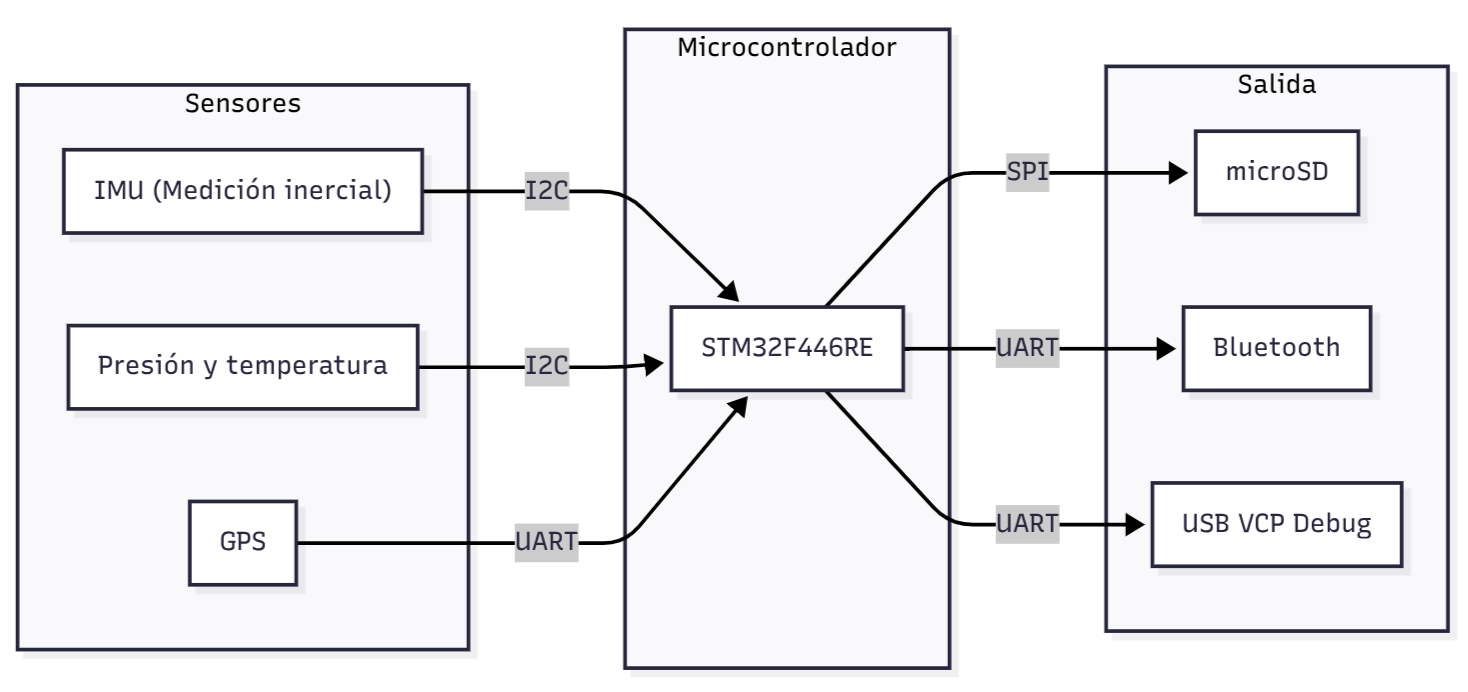
\includegraphics[width=0.92\textwidth]{Figures/cap2-interconexion-buses.png}
	\caption{Interconexión lógica entre el microcontrolador y los periféricos del prototipo.}
	\label{fig:interconexion-buses-cap2}
\end{figure}

El diagrama condensa las relaciones de la tabla~\ref{tab:componentes-externos}. El GNSS y el módulo Bluetooth emplearon UART dedicadas, la unidad inercial compartió el bus I2C1 con el integrado central, y la microSD se accedió por SPI2. El puerto serie del ST-LINK quedó disponible para depuración sin formar parte del lazo de telemetría en el vehículo.

%----------------------------------------------------------------------------------------
\section{Sistema operativo y middleware}
\label{sec:rtos-middleware}

El firmware del prototipo se ejecutó sobre un sistema operativo de tiempo real (RTOS, \textit{Real-Time Operating System}). Se empleó FreeRTOS \citep{freertos} integrado en el árbol de middleware de STM32Cube, con el planificador preemptivo por prioridades para asegurar plazos acotados en adquisición, registro y enlace inalámbrico. La arquitectura concurrente del firmware y el reparto en tareas y colas de mensajes se detallan en el capítulo~\ref{Chapter3}.

\subsection{Capas de software de terceros}

Sobre el kernel RTOS se integraron las siguientes piezas de soporte:

\begin{itemize}
	\item CMSIS y HAL de STM32, generados con STM32CubeMX a partir del paquete de firmware STM32Cube para la familia F4, para acceso a GPIO, temporizadores, DMA y periféricos serie.
	\item FreeRTOS, con APIs de tareas, colas, semáforos y temporizadores de software, como base del planificador y de la comunicación entre módulos de firmware.
	\item FatFs, integrado en el árbol de middleware del proyecto, para operar sobre la tarjeta microSD con partición FAT32.
	\item Herramientas de verificación en el host (Ceedling \citep{ceedling} y Unity \citep{unity}) para pruebas unitarias de componentes de firmware, sin formar parte del binario embarcado.
\end{itemize}

La capa HAL abstrajo los registros de hardware en rutinas de configuración y ocultó los detalles del fabricante detrás de tipos comunes para UART, I2C y SPI. CMSIS aportó definiciones del núcleo Cortex-M y vectores de interrupción coherentes con la documentación del fabricante. Las llamadas al sistema de archivos se ejecutaron desde las tareas de aplicación, con exclusión mutua frente a otras tareas que pudieran disputar el mismo medio.

\subsection{Aplicación móvil y servicios en el teléfono}

En el lado del teléfono móvil se empleó una aplicación web progresiva \citep{mdn_pwa} desarrollada con React \citep{react} y Vite \citep{vite}. La comunicación con el prototipo utilizó la API Web Bluetooth \citep{w3c_web_bluetooth} del navegador, que expuso el perfil del módulo HC-10 hacia la capa de presentación (mapas y visualización de telemetría). Ese modelo evitó distribuir un binario nativo por medio de las tiendas de aplicaciones y permitió iterar la interfaz con las mismas tecnologías empleadas en el ecosistema web. Los mapas se apoyaron en la biblioteca Leaflet \citep{leaflet} de código abierto. La interpretación de las tramas recibidas por BLE residió en el cliente y no en el microcontrolador.

La figura~\ref{fig:capas-software-cap2} resume las relaciones entre las capas de software del microcontrolador y el cliente móvil. El detalle de tareas, colas de eventos, drivers y formatos de registro se describe en el capítulo~\ref{Chapter3}.

\begin{figure}[htbp]
	\centering
	% Fuente editable: Figures/cap2-capas-software.mmd (mermaid-cli)
	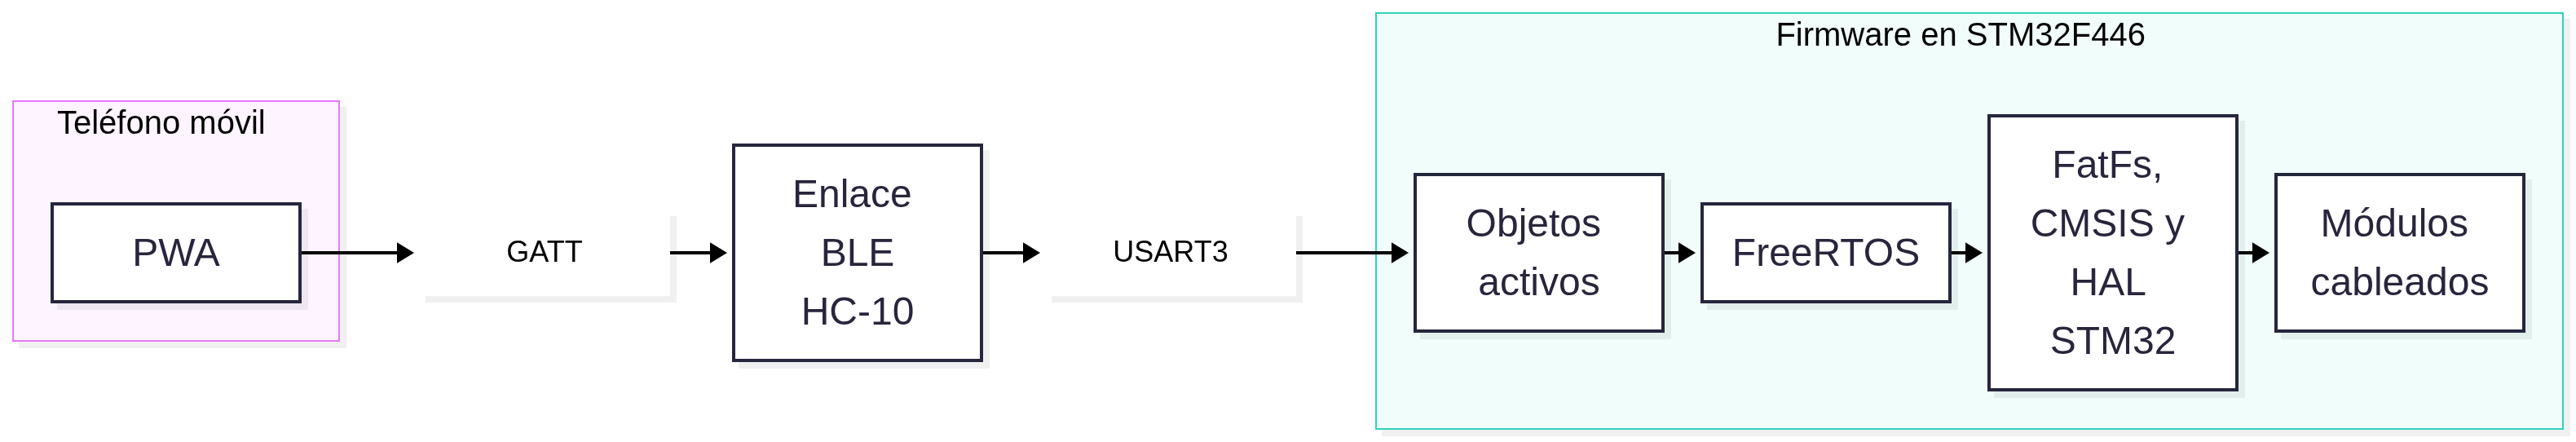
\includegraphics[width=0.95\textwidth]{Figures/cap2-capas-software.png}
	\caption{Capas de software en el microcontrolador y en el teléfono móvil.}
	\label{fig:capas-software-cap2}
\end{figure}

%----------------------------------------------------------------------------------------
\section{Protocolos y buses de comunicación}
\label{sec:protocolos-buses}

Los enlaces físicos entre el STM32F446 y los módulos externos se implementaron con tres familias de interfaz habituales en adquisición de sensores y almacenamiento local. En la tabla~\ref{tab:parametros-buses} se resumen las instancias configuradas en el prototipo.

\begin{table}[H]
	\centering
	\caption[Parámetros de buses]{Parámetros de los buses serie y paralelos configurados en el prototipo.}
	\setlength{\tabcolsep}{4pt}
	\begin{tabularx}{\textwidth}{@{}>{\raggedright\arraybackslash}p{1.45cm}>{\raggedright\arraybackslash}p{1.95cm}>{\raggedright\arraybackslash}p{2.35cm}>{\raggedright\arraybackslash}X@{}}
		\toprule
		\textbf{Bus} & \textbf{Periférico} & \textbf{Tasa / modo} & \textbf{Rol en el sistema} \\
		\midrule
		USART1 & NEO-M8N & 9600 baudios & Recepción de tramas NMEA por DMA a buffer circular \\
		USART2 & ST-LINK VCP & 115200 baudios & Consola de depuración hacia el host \\
		USART3 & HC-10 (BLE) & 9600 baudios & Enlace serie transparente con el teléfono \\
		I2C1 & LSM6DSO & 100~kHz, maestro & Lectura periódica de registros de la IMU \\
		SPI2 & microSD & Modo maestro, DMA & Almacenamiento de ficheros CSV vía FatFs \\
		\bottomrule
	\end{tabularx}
	\label{tab:parametros-buses}
\end{table}

En la comunicación UART asíncrona se configuraron tres instancias USART para el GPS (9600 baudios), la depuración por ST-LINK (115200 baudios) y el módulo Bluetooth (9600 baudios). El enlace con el receptor NEO-M8N se apoyó en sentencias NMEA para obtener coordenadas y tiempo de referencia. La recepción en USART1 se realizó por DMA hacia un buffer circular, de modo de reducir la carga de interrupciones ante ráfagas de tramas. Las sentencias se acumularon en ese buffer y se descartaron tramas incompletas antes de interpretarlas. La depuración y el módulo HC-10 operaron sin DMA, con una carga de tráfico inferior. En el módulo BLE el UART actuó como túnel serie hacia el controlador CC2541. No se implementó un protocolo propietario encima de los octetos en el firmware embarcado.

El bus I2C1 conectó la IMU LSM6DSO en modo maestro a 100~kHz. Los registros del sensor se accedieron mediante direccionamiento de 7 bits y lecturas de bloques para aceleración y velocidad angular.

El bus SPI2 enlazó la tarjeta microSD en modo maestro con una línea de selección de esclavo dedicada. Las transferencias en bloque hacia la tarjeta se apoyaron en DMA, alineadas con lo descrito en la sección~\ref{sec:plataforma-hardware}. Las operaciones de lectura y escritura se tradujeron a llamadas al middleware FatFs sobre ficheros en formato CSV. Se asumió el uso de una partición FAT32 y un tamaño de cluster compatible con tarjetas de uso general de hasta 32~GB.

A nivel de aplicación móvil, el intercambio con el usuario se realizó mediante el perfil GATT expuesto por el módulo (servicio y característica de datos serie), mientras que la persistencia local en el vehículo dependió del sistema de archivos FAT ya referido en el microcontrolador. Las capas descritas en este capítulo se integran en el diseño detallado del capítulo~\ref{Chapter3}, donde se explicitan los módulos de firmware y los formatos de registro adoptados.